%----------------------------------------------------------------------------
\chapter{The Language module and two examples}
%----------------------------------------------------------------------------
\section{The Language module}
The Language module consists of only one class - the Language class - which encapsulates the Lexer and Parser classes. It has two getters - one for the Lexer and one for the Parser, and a method to build and return the AST from the raw source code string.
The module exports the Language class, which has the Lexer and Parser classes as subclasses too.
\section{Examples}
I have written two example language modules to test the modules - one is a math expression parser, and the other is a very small subset of the Logo programming language - a for cycle, and the drawing statements are accepted, and of course the parameters can be math expressions.
\subsection{The math parser}
The way I imagined people could create language modules is by extending the Language class - and this is what I have done in this case. In the constructor I initialize the Lexer token classes, and the parser with the BNF grammar. I added two more methods - an executeOne and an execute method. The execute method builds the AST using the parser's parse method, and calls executeOne on the main node. The executeOne method then recursively executes the subtrees of the nodes - it checks for known types based on the names of the token classes, and parses the integers and floats into their numerical values. If the current node is not a terminal, then it first calls itself on that node to determine it's value. Once all the numerical parameters are ready, it does the calculation, and returns the resulting number. This is done using switch statements to handle each rule in it's own way.

\begin{lstlisting}[frame=single]
const Language = require('../lib/language')
const { Lexer, Parser } = Language

class BasicMath extends Language {
  constructor() {
    super()
    
    this.lexer.addTokenClasses([
      new Lexer.TokenClass('int', /[0-9]+(?![0-9]*\.)/),
      new Lexer.TokenClass('float', /[0-9]+\.[0-9]+/),
      new Lexer.TokenClass('char', /\S/)
    ])
    
    this.parser.fromBNF(
      `<S> ::= <S> <SEP> <E> | ""
      <SEP> ::= "," | "" | <Token-EOL>
      <E> ::= <E> <PM> <T> | <T>
      <T> ::= <T> <MD> <H> | <H>
      <H> ::= <H> "^" <F> | <F>
      <PM> ::= "+" | "-"
      <MD> ::= "*" | "/"
      <F> ::= "(" <E> ")" | <Token-int> | <Token-float>`
    )
  }
  
  executeOne(node) {    
    if (node.rule.class !== undefined) {
      switch (node.rule.class.name) {
        case 'int':
          return parseInt(node.rule.value)
          break;
        case 'float':
          return parseFloat(node.rule.value)
          break;
        default:
          return node.rule.value
      }
    }
    
    let parameters = node.children.map(child => {
      return this.executeOne(child)
    })
    
    switch (node.rule.name) {
      case 'E': case 'T':
        switch (parameters[1]) {
          case '-':
            return parameters[0] - parameters[2]
            break
          case '+':
            return parameters[0] + parameters[2]
            break
          case '*':
            return parameters[0] * parameters[2]
            break
          case '/':
            return parameters[0] / parameters[2]
            break
          default:
            throw Error('Unknown rule')
        }
        break
      case 'H':
        return Math.pow(parameters[0], parameters[1])
        break
      case 'F':
        return parameters[0]
        break
      case 'S':
        if (parameters.length === 1)
          return parameters[0]
        return parameters[0] + ', ' + parameters[parameters.length - 1]
        break
      default:
        throw Error('Unknown rule')
    }
  }
  
  execute(code) {
    let ast = this.buildAST(code)
    return this.executeOne(ast[0])
  }
}

module.exports = new BasicMath()
\end{lstlisting}

I have added some extra rules to verify that the parser can handle optional rules (rules with $\epsilon$ as an alternative) and left-recursion. By carefully constructing the grammar I have ensured that the operator precedence is as it should be ($nth power > */ > +-$).

\begin{lstlisting}[frame=single]
const BasicMath = require('./examples/math')
global.BasicMath = BasicMath
console.log(
  BasicMath.execute(`10 ^ ((10 - 5 + 4) / (6 - 3)), 10 22/10
  432.432/10`)
)
\end{lstlisting}

Running this piece of code results in the following: \lit{1000, 10, 2.2, 43.2432}, which is indeed the expected output.

\subsection{The Logo subset parser}
The way the Logo subset parser is constructed is similar to the math expression parser. 

It uses the following grammar:
\begin{grammar}

<Program> ::= <Program> <Expression> \alt \lit{}

<Expression> ::= <Command> \alt <For>

<Command> ::= <Command-name> <Math>

<Command-name> ::= \lit{f} \alt \lit{b} \alt \lit{l} \alt \lit{r} 

<For> ::= \lit{for} <Math> \lit{[} <Program> \lit{]}

<Math> ::= <Math> <PM> <T> \alt <T>

<T> ::= <T> <MD> <H> \alt <H>

<H> ::= <H> "^" <F> \alt <F>

<PM> ::= \lit{+} \alt \lit{-}

<MD> ::= \lit{*} \alt \lit{/}

<F> ::= \lit{(} <Math> \lit{)} \alt <Token-int> \alt <Token-float>

\end{grammar}

\begin{lstlisting}[frame=single]
const Logo = require('./examples/logo')
global.Logo = Logo
\end{lstlisting}

By providing a callback parameter, and implementing simple drawing on a HTML5 canvas in JavaScript, if we bundle the interpreter script and handle the necessary things in the browser, we can actually create drawings fairly easily.

\begin{lstlisting}[frame=single]
logo.execute(`for 360 [f 2 r 1] for 10^2+50 [f 321 r 121 for 2 [r 1 l 1]]`)
\end{lstlisting}

This code generates the following image:

\begin{center}
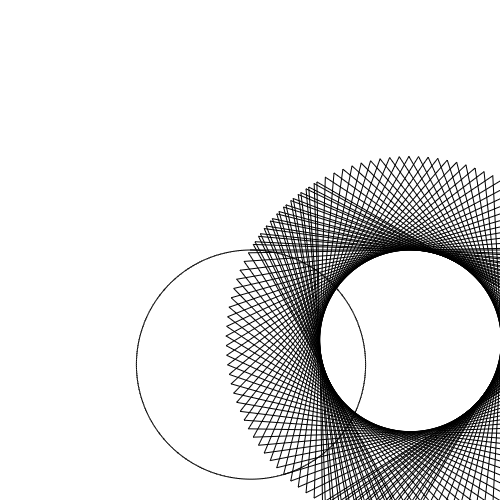
\includegraphics[width=60mm,keepaspectratio]{figures/logo.png}
\end{center}